\chapter{Kryptologie}

\section{Grundbegriffe und einfache Verfahren}
\begin{figure}[h]
	\centering
	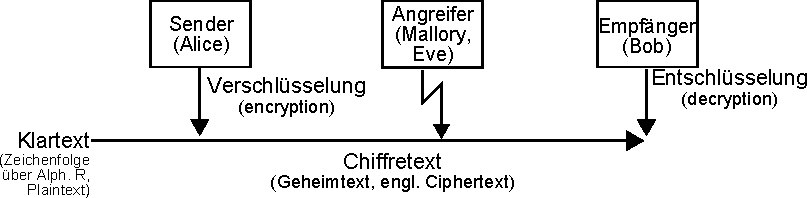
\includegraphics{./img/krypto_schaubild.pdf}
	\caption{Schaubild der Kryptologie}
	\label{img:Schaubild}
\end{figure}

\subsection{Verschl�sselung erfordert}

\begin{itemize}
	\item[-] Verschl�sselungsverfahren, Algorithmus (Funktion)
	\item[-] Schl�ssel $k_{e}$ (encryption key)
\end{itemize}

\[
	E(m,k_e)=c
\]	
$E$=Verschl�sselungs Funktion, $m$=Klartext, $c$=Chiffretext
\[
	E(m_1,k_e) \neq E(m,k_e)\ fuer \ m_1 \neq m_2
\]
\[
	D(c,k_d)=m
\]	
($k_d$ zu $k_e$ geh�riger Dechiffrierschl�ssel!)\\
$k_d=k_e$ (oder $k_d$ leicht aus $k_e$ zu berechnen):\\
\textbf{symmetrisches Verschl.verf.}, ansonsten \textbf{asymm. Verschl.verf.}. Ist $k_d$ nur sehr schwer (oder garnicht) zu $k_e$ berechenbar, so kann $k_e$ ver�ffentl. werden:\\
\textbf{Public-Key-Verfahren}.

\subsection{Beispiel f�r (nicht sicheres) symm. Verfahren}

\begin{itemize}
	\item[a)] $R=S=\left\{0,1,\ldots,25\right\}$\\
	Verfahren: Verschiebechiffre\\
	Schl�ssel: $i \in \left\{0,1,\ldots,25\right\}$\\
	Verfahren $ x \in \R \longrightarrow x+i\, mod\, 26=y$\\
	$y\longmapsto y-i\, mod\, 26 = y$\\
	$m=x_1 ... x_2 \longrightarrow  c = (x_1 + i\, mod\, 26) \textbf{}\ldots (x_n +i\, mod\, 26)$, $E(m,i)$\\
	Unsicher, weil Schl�sselmenge klein ist (Brute Force Angriff).
	\item[b)] R,S, Schl�sselmenge=Menge aller Permutationen von $\left\{1,\ldots,25\right\}=S_{26}$\\
	Verschl.: W�hle Permuation $\pi$\\
	$x \in \R \longrightarrow \pi (x)=y$\\
	Entschl.: $y \longrightarrow \pi^{-1}(y)=x$\\
	$m=x_1 \ldots x_r \rightarrow c=\pi(x_1)\ldots\pi(x_r)$\\
	$\begin{pmatrix}
  0 & 1 & 2 & \ldots & 25 \\
  3 & 17 & 4 & \ldots & 13
	\end{pmatrix}
	\longrightarrow \pi(0)=3$, u.s.w.\\
	Anzahl der Permutationen: $\left|{S_{26}}\right|=26!\approx4\cdot10^{26} \longrightarrow$ Brute-Force Angriff nicht mehr m�glich! \\
	Warum? Man muss im Schnitt 50\% der Permutationen testen. Angenommen man k�nnte $10^12$ Perm. pro Sekunde testen.\\
	Aufwand: $2\cdot10^{14}$ Sekunden $\approx 6.000.000$ Jahre\\
	Trotzdem unsicher!\\
	Grund: Charakteristiches H�ufigkeitsverteilung von Buchstaben in nat�rlichspr. Texten.
\end{itemize}
Verfahren beinhalten viele Verschl�sselungsm�glichkeiten, abh�ngig von der Auswahl des Schl�ssels.\\
Verfahren bekannt, aber Schl�ssel $k_d$ geheim!\\
\subsection{Prinzip von Kerkhoffs (1835-1903)}
Sicherheit eines Verschl�sselungsverfahren darf nicht von der Geheimhaltung des Verfahrens, sondern nur von der Geheimhaltung des verwendeten Schl�ssels abh�ngen!
%
%	Ende Stunde vom 29.10.2009
%
\\\\
Kryptologie besteht aus Kryptographie (Entwurf) und der Kryptoanalyse (Angriff).
Angriffserfolge:
\begin{itemize}
	\item[-] Schl�ssel $k_d$ wird gefunden
	\item[-] Eine zu der Dechiffrierfunktion $D(\cdot,k_d)$ �quivalente Funktion finden ohne Kenntnis von $k_d$
	\item[-] gewisste Chiffretexte werden entschl�sselt
\end{itemize}
\subsection{Arten von Angriffen}
\begin{itemize}
	\item[-] Ciphertext-Only Angriff
	\item[-] Known-Plaintext Angriff
	\item[-] Chosen-Plaintext Angriff
	\item[-] Chosen-Ciphertext Angriff
\end{itemize}